\chapter{Механика}

%================================================================================
% ЦЯЛОСТЕН МОДЕЛ
 
\section{Цялостен модел на робота}

Както е описано в предишната глава, дизайна на бойния робот е вдъхновен от робота SawBlaze. Материала, който е използван за изграждането на прототипа на проекта е два милиметра дебела студено валцована въглеродна стомана DC01. Механичната конструкция на робота може да бъде разделена на два основни компонента - шасито, в което седят почти всички елементи, и механичната ръка, на която е закрепено оръжието.  

\begin{figure}[H]
    \centering
    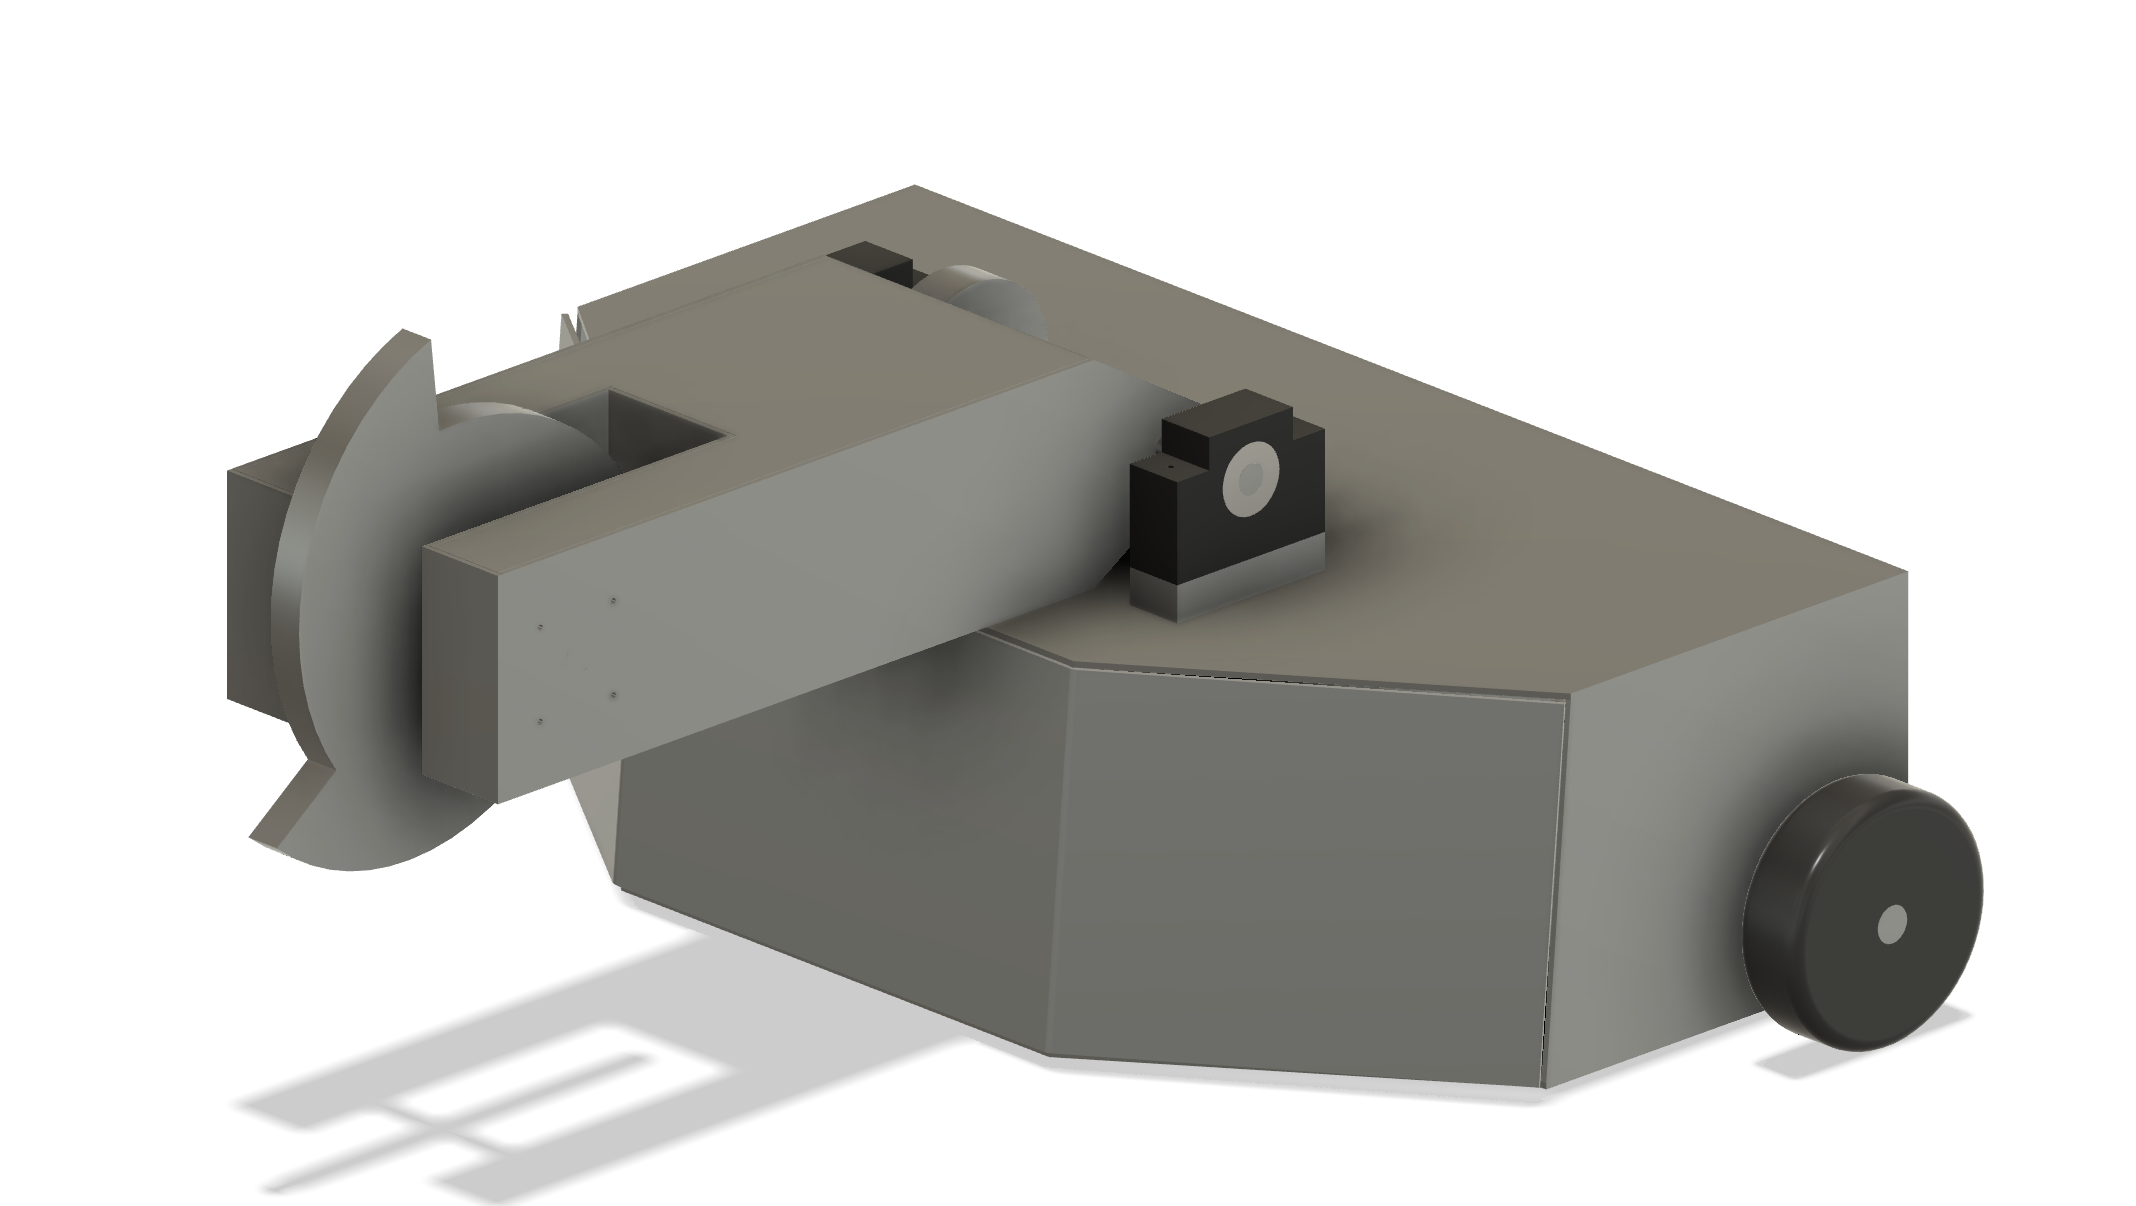
\includegraphics[width=1.1\linewidth]{images/robot-home.png}
    
    \caption{3D макет на бойния робот}
    \label{fig:robot-home} 
\end{figure}

%================================================================================
% ЗАДВИЖВАНЕ

\section{Задвижване на робота}
\label{sec:motion}

По време на проектирането на механиката на боен робот първият проблем, който трябва да бъде разгледан е как той ще се придвижва по арената. След направеното проучване в \cref{sec:motion-types} бе установено, че най-ефективният метод е диференциалното задвижване с колела. По дизайн роботът има две задвижващи колела отдвете си страни и още две допълнителни пасивни колела, които го балансират и му помагат да се движи по-добре. Всяко от задвижващите колела е с външен диаметър 80мм и ширина 12мм. Използваните мотори за тяхното задвижване са CHANCS 895 DC.

\begin{figure}[H]
    \centering
    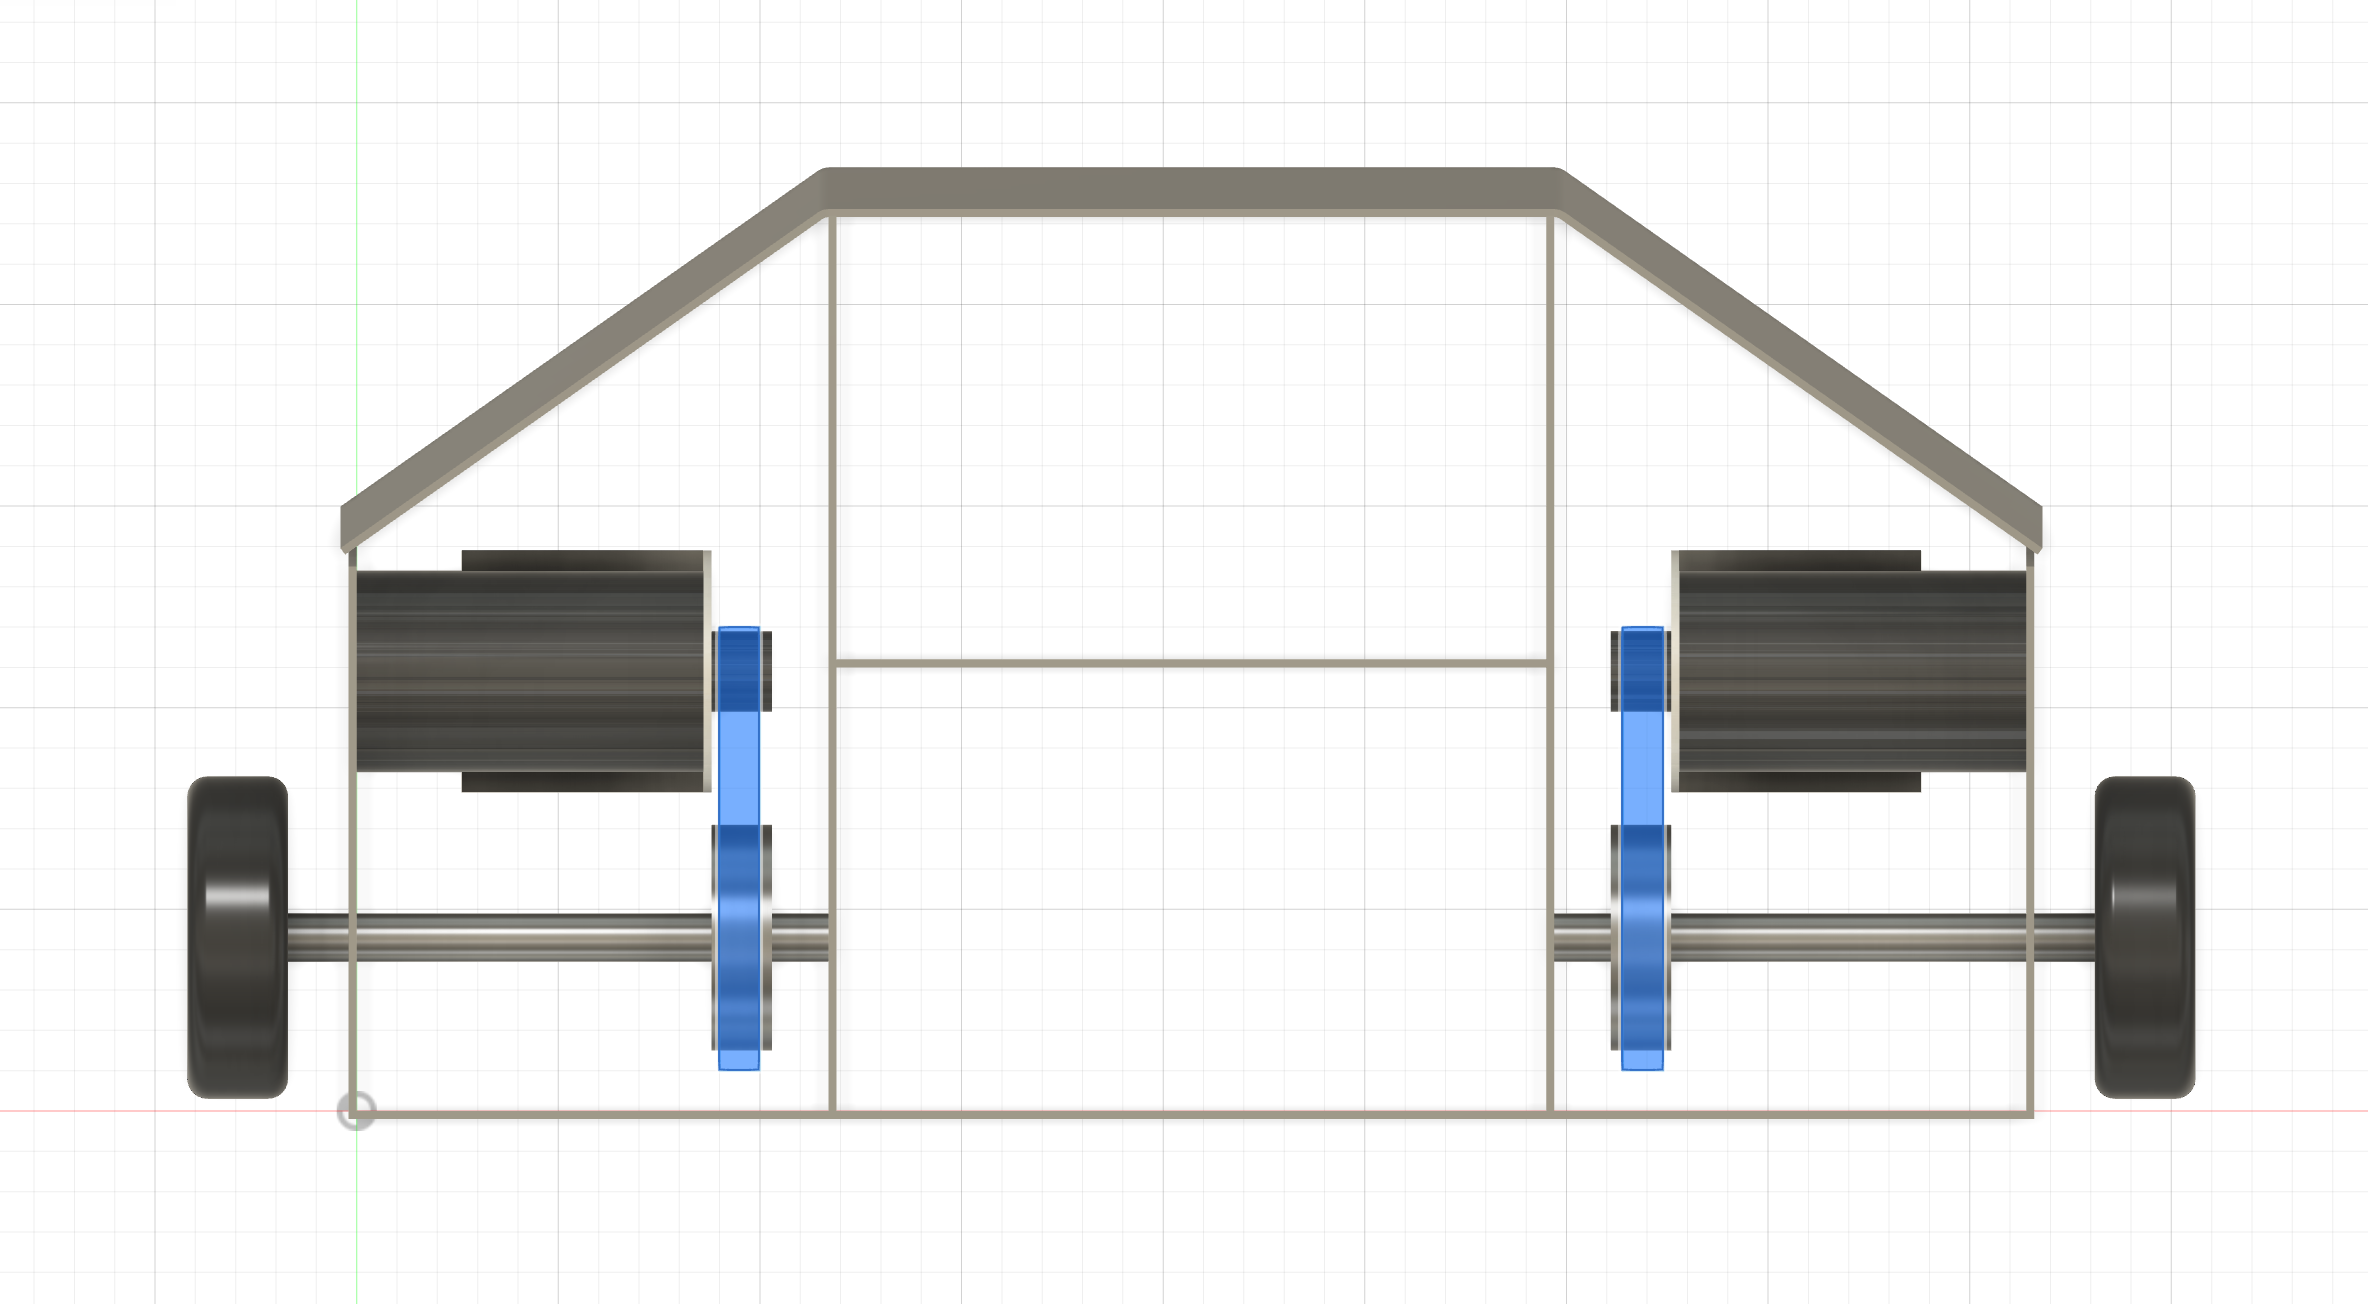
\includegraphics[width=\linewidth]{images/motion.png}
    
    \caption{Схема на задвижването на бойния робот}
    \label{fig:motion} 
\end{figure}

За да може батълбота, който тежи приблизително 18kg, да се задвижва от две колела трябва да бъде пресметнато какъв въртящ момент трябва да достига до всяко от тях
\footnote{Изчисленията са извършени като се приема, че роботът се движи на равна повърхност}
. За целта на изчисленията приемаме, че двете активни колела ще понасят цялото тегло на робота. Понеже на двете колела лежи тежестта от 18kg, означава, че всяко колело изпитва натиска от 9kg или еквивалентните им 88,29N. Коефициента на триене между колелата и пода на арената варира между 0,75 когато робота е в покой и 0,65 когато е в движение. Следователно най-голямата сила на съпротивление, която всяко колело може да генерира без самото колело да се върти е 88,29N х 0.75 = 66,2175N. След като диаметъра на колелото е 80мм следва, че радиусът му е 40мм или 0,04м. Следователно минималният въртящ момент, който позволява на колелата да се въртят е равен на 66,2175N x 0,04m = 2,6487Nm. Следователно минималният въртящ момент, който мотора трябва да достави на колелото е 2,6487Nm, но по време на въртенето си той има само 0,735Nm.

Поради тази причина се налага да се направи редукция на скоростта на мотора за да се увеличи неговия въртящ момент. За да се изчисли каква трябва да бъде нужната редукция трябва да се намери отношението на необходимият въртящ момент и този, който може да бъде генериран. Редукцията, която се получава, че трябва да бъде реализирана между мотора и колелото е минимум 2,6487Nm / 0,735Nm = 3,6.

Начинът, по който е реализирано диференциалното задвижване е като всяко от активните колела бива задвижвано от различен мотор. Връзката между тях е реализирана, чрез зъбчат ремък с ширина 10мм. За да се постигне необходимата редукция, отношението на зъбите на ремъчните ролки на осите на колелата и тези на моторите трябва да бъде равно на нея. Поради това използваните ролки на моторите са с по 10 зъба, а другите са с по 36 зъба. С цел намаляване на триенето между осите на колелата и стените, осите са захванати с лагери в специално изработените за целта лагерни опори, закрепени за стените.

%================================================================================
% РЪКАТА

\section{Задвижване на ръката}

Първата специфична функционалност на разработения боен робот е начина, по който механичната ръка се върти около оста си и се задържа на позицията, на която и бива зададено да седи. Тази задача бива изпълнена чрез употребата на стъпков мотор Nema 24.

За да може ръката да се върти около оста си първо трябва да бъде изчислено какъв въртящ момент ще бъде необходим за целта. Тежестта на ръката е приблизително 4kg, което означава, че силата която е нужно да бъде приложена за да може тя да се завърти е 39,24N. За да пресметнем колко е необходимият въртящ момент за нейното завъртане е необходимо получената сила да бъде умножена по дължината на ръката, която е 240мм(0,24м). По този начин получаваме, че трябва да бъдат приложени 39,24N х 0,24м = 9,4176Nm. Употребеният стъпков мотор може да задържа на една позиция само товари, които изискват въртящ момент 3,1Nm или по-малко, от което следва, че се налага да бъде приложена минимална редукция от 3,03 за да може да бъде реализирано въртенето на ръката.

\begin{figure}[H]
    \centering
    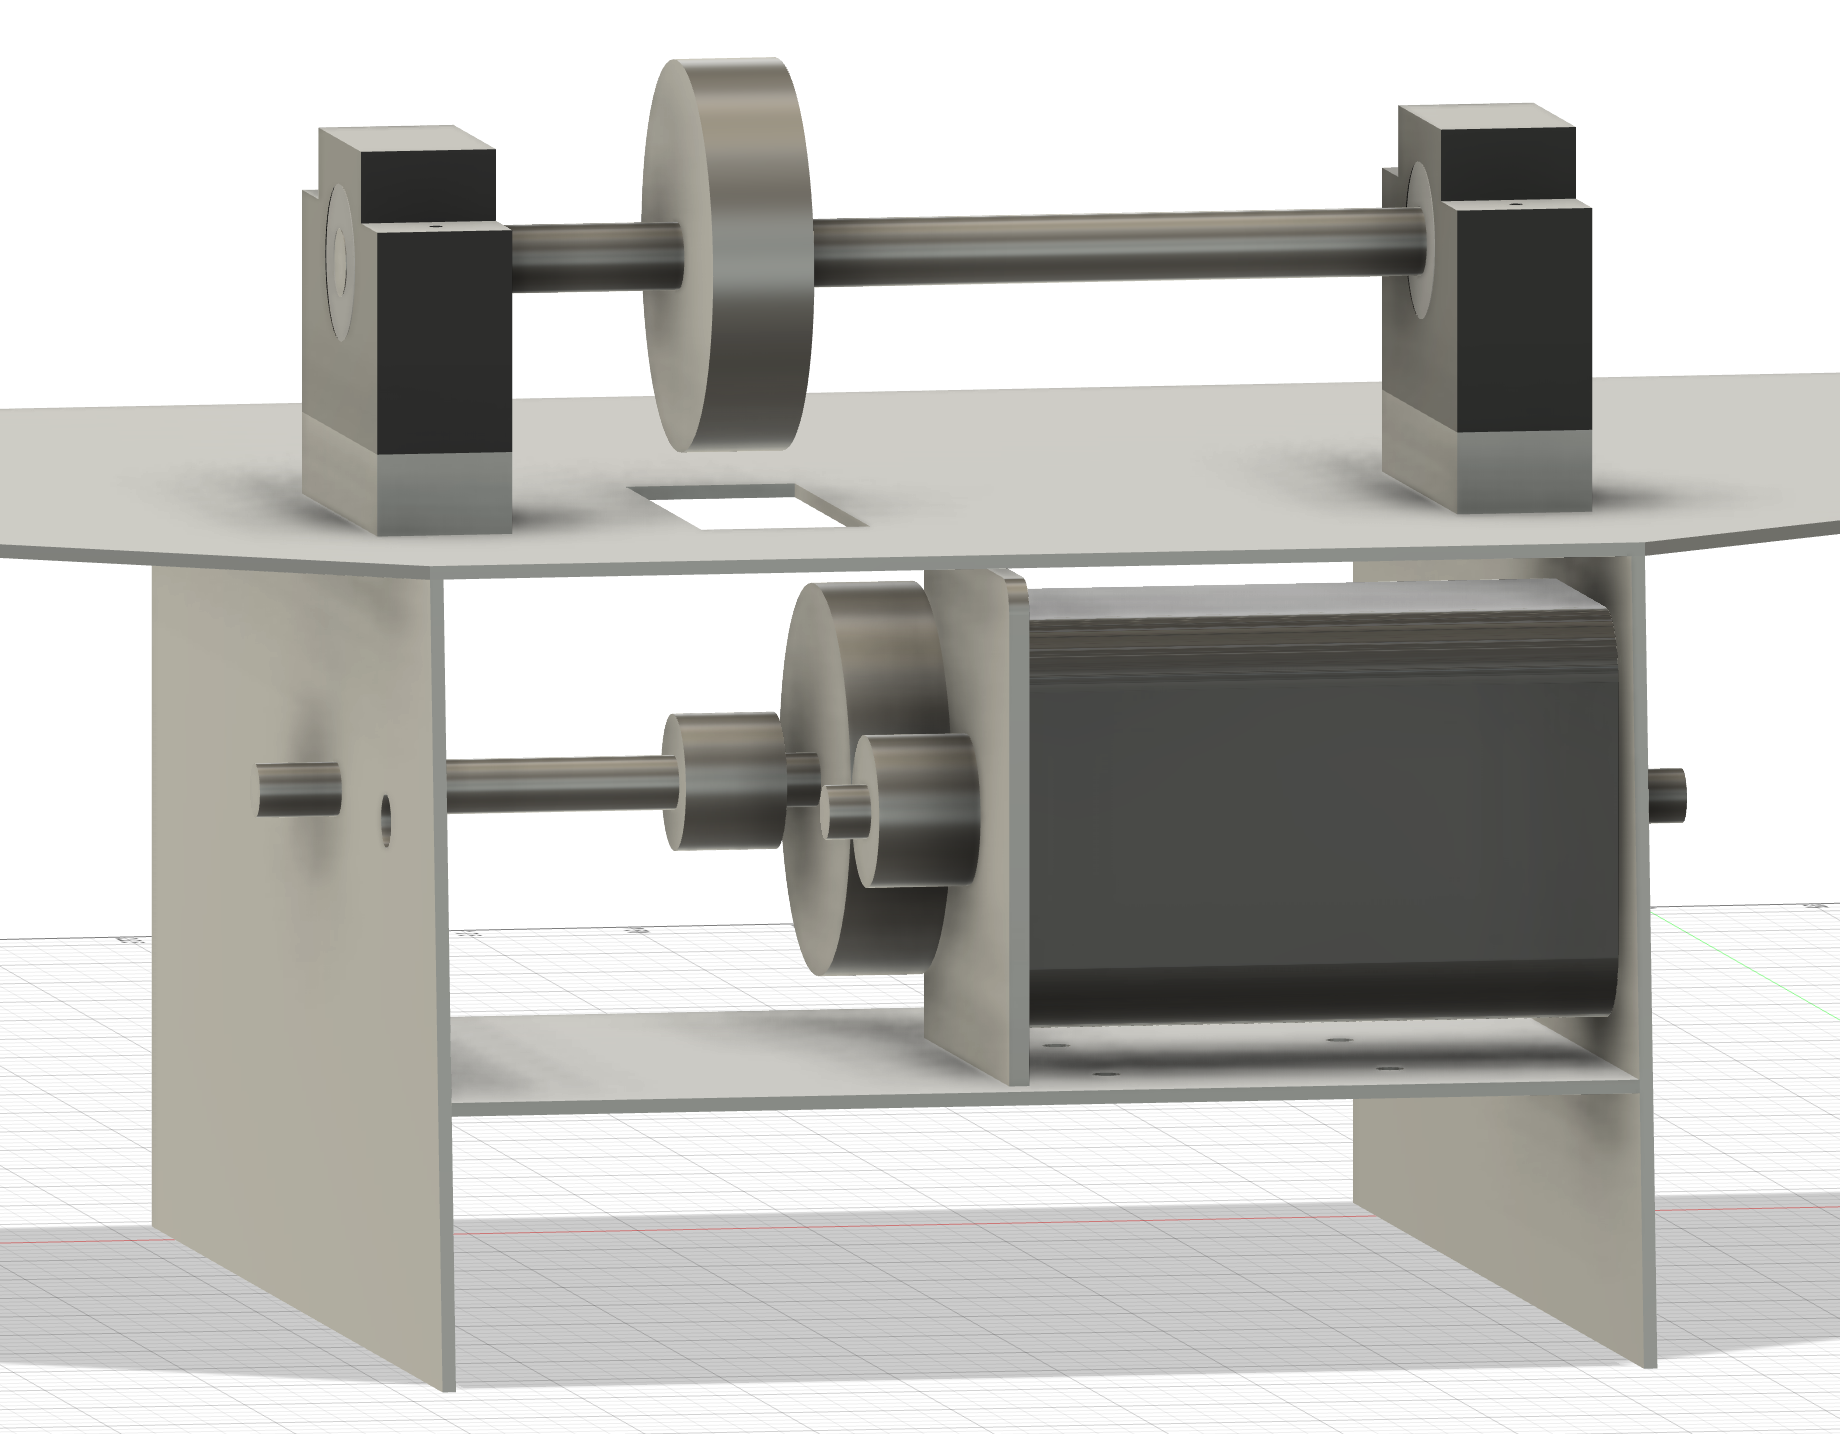
\includegraphics[width=\linewidth]{images/hand-movement.png}
    
    \caption{Схема на задвижването на механичната ръка}
    \label{fig:hand-movement} 
\end{figure}

Начинът, по който е осъществено завъртането на ръката е като тя бива захваната за своята ос така, че чрез завъртането на оста ръката да бъде придвижена заедно с нея. Предаването на движението от стъпковия мотор към оста на ръката е постигнато посредством зъбни ремъци. С цел максималното увеличение на приложената редукция е поставена спомагателна ос между мотора и оста на ръката. По този начин се получават две редукции на движението на мотора. Първата бива от мотора към спомагателната ос, като поставената ролка на мотора има 12 зъба, а тази на спомагателната ос 36 зъба. Постиганата редукция чрез тази връзка е 3. Втората редукция бива от спомагателната ос към оста на ръката и използваните ролки са в същото отношение като тези в предишната предавка. Резултатът от двете връзки е, че общата редукция на скоростта на въртене на мотора се получава да бъде умножението на двете, от които е съставена, което я прави 9. За намаляване на съпротивлението по време на въртенето си са поставени лагерни опори в краищата на двете оси.


%================================================================================
% ОРЪЖИЕТО

\section{Задвижване на оръжието}

Друг проблем, който трябва да бъде решен по време на проектирането на механиката на всеки боен робот е по какъв начин неговото оръжие ще се задвижва. Както е описано в точка \cref{sec:block-schemas} оръжието, което се използва в разработения проект е 180-милиметров диск с ширина 8мм и специфична форма. Формата на диска може да бъде видяна на фигура \cref{fig:disk}. Той е захванат за своята ос така, че чрез завъртането на оста и диска да се върти заедно с нея. Използваният мотор за движението на оръжието е CHANCS 895 DC. Начина, по който е реализирано предаването на движението от мотора до оста на диска е посредством плосък ремък. Избран е плосък ремък за тази цел, а не зъбчат поради причината, че при удар ремъка и мотора трябва отведнъж да спрат своето движение, което често може да доведе до прескачане на зъби на зъбчатия ремък и тяхното ронене. В тези ситуации плоския ремък няма да се амортизира по този начин, а само ще се приплъзне леко по своите ролки. Реализирана е и редукция от 5 на скоростта на тази предавка поради високата скорост, с която би се въртял диска. С цел намаляване на съпротивлението по време на въртенето си в краищата си оста на диска е поставен в лагерни опори, които са застопорени за стените на ръката.

\begin{figure}[H]
    \centering
    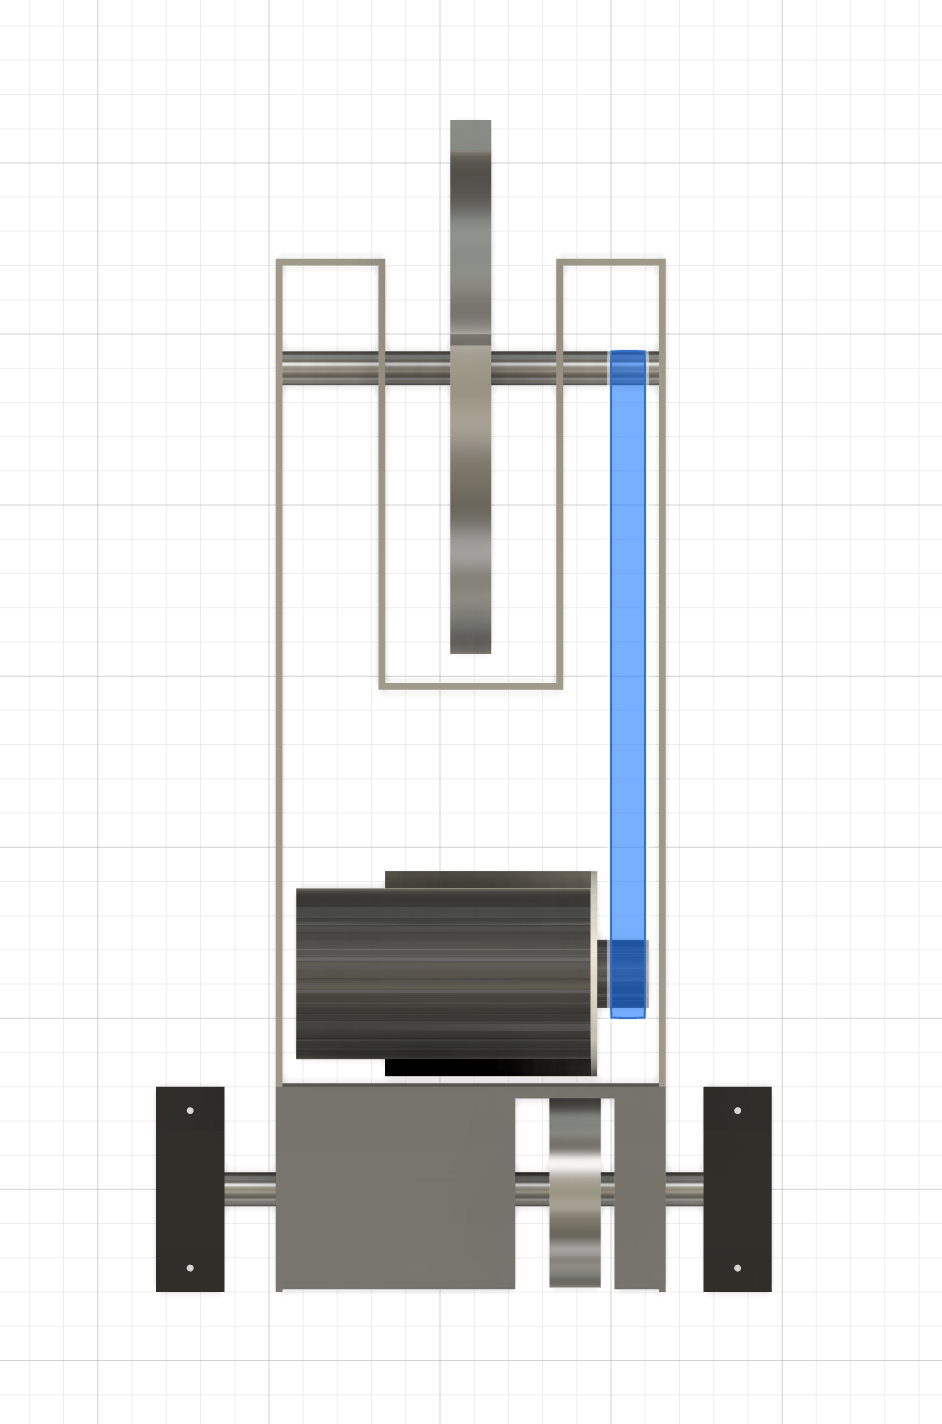
\includegraphics[width=0.8\linewidth]{images/hand-inside.png}
    
    \caption{Схема на задвижването на оръжието}
    \label{fig:hand-inside} 
\end{figure}
